% !TeX root = ../main.tex

\chapter{QD-LED中氧化锌类电子传输层研究}
\section{引言}
2011年,Qian等人将ZnO纳米粒子材料作为电子传输层,开发的基于ZnO传输层的溶液法器件结构是目前最广泛采用的QLED器件结构\cite{qian2011stable}。Qian等人证明了ZnO具有较为理想的高电子迁移率,相较于此前ETL材料存在较大的差距,在当时实现了QD-LED器件性能的巨大突破。目前,研究人员在此基础上实现了进一步优化,最为常见的是在ZnO中做金属阳离子掺杂处理,特别是Mg掺杂的ZnO纳米颗粒,可以说是目前高性能QD-LED器件电子传输层的不二选择。目前可以确定的是,Mg的掺杂可以改变ZnO的能级结构,并且适当降低电子注入速率。以实现更好的载流子注入平衡。此外,对于Mg掺杂的优势还有一些猜想,比如可能在与量子点接触时降低了量子点的猝灭,可能会降低热电子的注入数目,可能导致注入电子的能量的降低,可能会与ZnO形成特殊晶格结构等等,但目前还没有定数。此外,事实上目前研究人员对于ZnO纳米粒子都还存在诸多疑惑,我们知道ZnO纳米粒子具有较大的比表面积,因此不可避免的存在大量悬空键,自身非常不稳定且极易产生缺陷,但是在正项老化后却实现了极高峰值的外量子效率和较长的使用寿命。目前对于ZnO的研究并不透彻且尚未找到能完美替代ZnO的材料,因此,尽可能弄清ZnO类电子传输层在QD-LED器件中的机理和行为非常重要,这也是我们本篇工作此前搭建紫外波段拓展的电激发瞬态激发吸收光谱仪的主要目的,在本章节,我们将展示目前我们得到的实验结果。
\section{氧化锌纳米粒子}
氧化锌是一种 n 型宽带隙(E$_g$ $\approx$ 3.3 eV)半导体材料,通常为六方纤锌矿结构(图\ref{fig:ZnO},其在z轴上交替堆叠四面体配位的 O$^{2-}$ 和 Zn$^{2+}$ 离子),晶格常数a = 0.32 nm,c = 5.52 nm,属于C6$_3$mc空间群和6mm点群。
\begin{figure}[ht]
	\centering
	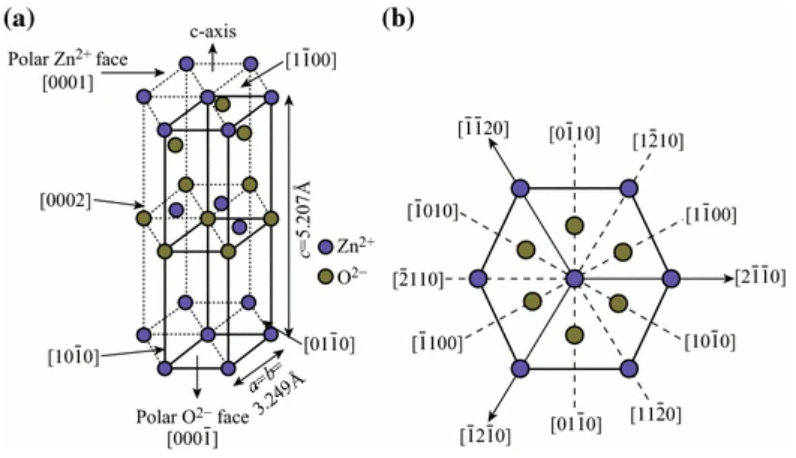
\includegraphics[width=.8\textwidth]{ZNO.png}
	\caption{ZnO晶胞和晶面\cite{kumar2015zinc}。}
	\label{fig:ZnO}
\end{figure}

\subsection{固有缺陷\cite{nadupalli2021defect}}
氧化锌主要存在五种固有缺陷:(1)氧空位(V$_O$),包含三个简并态V$^{2+}_O$、V$^{1+}_O$、V$^{0}_O$,氧空位的电荷态与晶格结构中的微观应力直接相关,晶格弛豫也会影响氧空位的形成能;(2)氧间隙(O$_i$),氧化锌中的氧间隙缺陷可能是单独存在的,也可能是由于另一个空位引起的弛豫而导致氧离子在晶格中发生位移,氧间隙的电子构型以2p$^4$,、2p$^5$、2p$^6$结尾,分别产生O$_i^0$、O$_i^−$、O$_i^{2-}$;(3)锌空位(V$_{Zn}$),单个V$_{Zn}$在氧化锌晶格结构中会产生四个具有六个电子的悬挂氧键,悬挂氧键的简并态表现出电子性,使V$_{Zn}$成为一种受体型缺陷,V$_{Zn}$的形成能较低,使其成为一个主要缺陷,同时也是一个补偿中心;(4)锌间隙(Zn$_i$),Zn$_i$在纤锌矿氧化锌结构中占据四面体或八面体位点,如果Zn$_i$位于四面体位置,它的近邻原子为一个 Zn 原子和一个 O 原子,距离为 0.83d(d为沿 z 轴的 Zn-O 键长度),如果Zn$_i$位于八面体位置,则有三个 Zn 原子和一个 O 原子,距离为 1.07d,相较于四面体位点更加稳定而有利。Zn$_i$的电子构型以 4s$^2$  结尾,由于电子成对,因此它是一个抗磁中心;(5)氢缺陷 (H$_O$):氢缺陷取代氧位点。与 V$_O$相比, H$_O$缺陷以稳定的单正电荷态出现,形成能较低,H$_O^+$电荷态作为浅施主,可以调节ZnO的电导率。

\begin{figure}[ht]
	\centering
	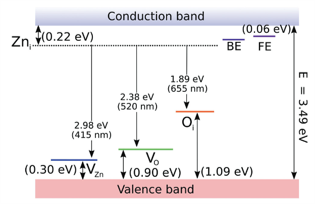
\includegraphics[width=.8\textwidth]{缺陷.png}
	\caption{ZnO固有缺陷能级示意图\cite{nadupalli2021defect}。}
	\label{fig:缺陷}
\end{figure}

V$_O$和V$_{Zn}$分别是表面缺陷和核心缺陷。V$_{Zn}^-$会产生一个空穴,它通过与晶格中的氧离子耦合产生一个孤立的O$^-$离子,从而产生有利于局域化的空穴。这种现象会导致晶格畸变,破坏局部点群对称性。O$^-$离子具有顺磁性,其 2p 壳层中缺少一个电子。由于这种离子与缺陷和晶格畸变有关,S = 1/2自旋与 2p 轨道的耦合很弱,导致自旋弛豫时间相当长。
\subsection{PL光谱}
图\ref{fig:PL}展示了ZnO量子点、ZnO纳米晶体和块体ZnO在室温下的PL 光谱,这里我们关注的是ZnO量子点的PL谱,可以看出,其主要存在两个峰,分别是380nm左右的紫外发射峰和540nm附近的可见光发射峰。紫外发射峰具有较高的能量,表现为一尖峰,其主要由ZnO的带间跃迁引起,即导带电子与价带空穴的辐射复合。在量子点中,量子限域效应会导致带隙增大,紫外峰发生蓝移。此外,量子点的表面钝化状态也会影响紫外发射强度。未钝化的表面缺陷可能导致非辐射复合,降低紫外峰强度;而良好的表面修饰(如有机配体包覆)可抑制缺陷态,增强紫外发射。而可见光发射峰能量较弱,表现为一宽峰,其主要与ZnO中的本征或外延缺陷有关,根据峰位差异通常有不同的解释:(1)绿色发射(~500-550 nm),通常归因于氧空位(V$_O$)相关的跃迁,氧空位在禁带中引入浅施主能级(约0.3-0.5 eV低于导带底),电子从导带或浅缺陷态跃迁至深能级(如V$_O^{+}$或V$_O^{2+}$)时发射绿光。(2)黄色/橙色发射(~550-600 nm),可能与锌空位(V$_{Zn}$)或氧间隙(O$_i$)有关。V$_{Zn}$作为受主缺陷(约0.5-0.8 eV高于价带顶),其与导带电子的复合可导致黄光发射。(3)此外,还可能受表面态影响,由于量子点的较高的比表面积导致表面悬挂键或吸附分子形成表面缺陷态,可能参与复合过程而贡献可见光发射。
\begin{figure}[ht]
	\centering
	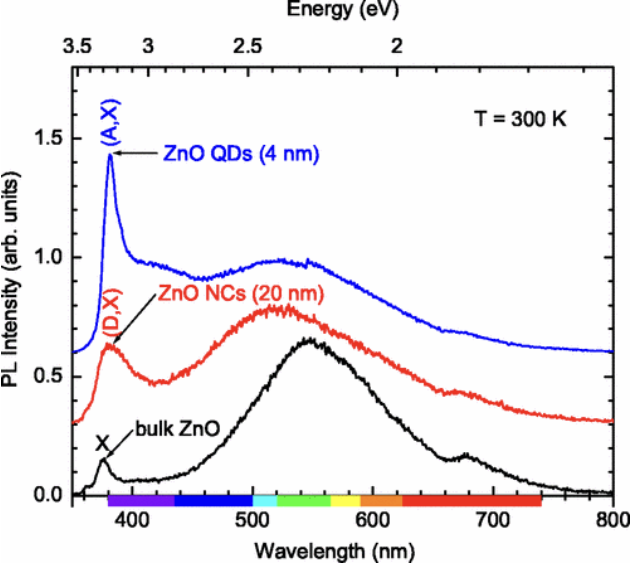
\includegraphics[width=.8\textwidth]{PL.png}
	\caption{ZnO 量子点、ZnO 纳米晶体和块体 ZnO(平面)的室温 PL 光谱\cite{PhysRevB.73.165317}。}
	\label{fig:PL}
\end{figure}
\subsection{制备方法}
氧化锌纳米粒子的制备方法主要包括固相法、气相法(化学气相氧化法、激光诱导化学气相沉积法、喷雾热解法)、液相法(包括直接沉淀法、均匀沉淀法、溶液-凝胶法、反胶团法、水热法)等\cite{GSYT200405013}。
\begin{figure}[ht]
	\centering
	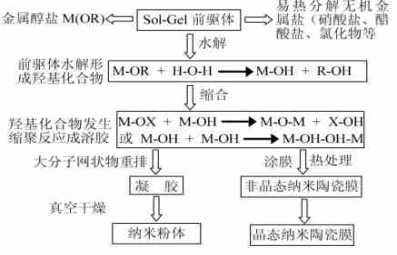
\includegraphics[width=.8\textwidth]{制备.png}
	\caption{Sol-Gel 法的工艺过程\cite{HXGY200903022}。}
	\label{fig:SG}
\end{figure}

在QD-LED领域中,制备氧化锌纳米粒子主要使用溶液-凝胶法(Sol-gel法)。前驱体选择硝酸锌(Zn(NO₃)₂·6H₂O)或醋酸锌(Zn(CH₃COO)₂·2H₂O),溶解在去离子水或乙醇中,NaOH或氨水作为沉淀剂溶液,在磁力搅拌下,将沉淀剂溶液逐滴加入锌盐溶液中发生水解、缩合化学反应,在溶液中形成稳定的透明溶胶体系,溶胶经陈化,胶粒间缓慢聚合,形成三维空间网络结构的凝胶。凝胶经过干燥、烧结固化制备出纳米亚结构的ZnO晶相。

溶液-凝胶法最大的优势是合成成本较低,并可通过控制溶液pH值、溶液浓度 、反应温度和时间参数制备粒径小 、分布窄 、均匀度高 、纯度高的纳米氧化锌颗粒\cite{GSYT200405013}。

\subsection{氧化锌纳米粒子电子传输层}
氧化锌纳米粒子作为QD-LED中电子传输层的天然优势在于:(1)氧化锌纳米粒子具有优异的电子迁移率(约200 cm²/V·s)和导电性,能够高效传输电子,减少器件中的电荷积累和界面复合损失。(2)ZnO的导带能级(约-4.3 eV)往往能较好的匹配量子点发光层的能级,降低了界面势垒,促进电子高效注入。(3)高透光率:ZnO在可见光区的透光率超过95\%,可以减少对发光层的光吸收干扰等等。

基于这些优势,氧化锌纳米粒子可以很好的胜任电子传输层的作用。但目前仍存在很多问题:(1)氧化锌电子传输层具有高电子迁移率,而目前HTL的空穴传输能力无法匹配,导致载流子注入不平衡,将导致非辐射复合的加剧,同时,电子泄露也是一个很麻烦的问题。(2)ZnO表面缺陷(如氧空位)可能成为激子猝灭中心,降低器件效率。(3)氧化锌层的厚度对器件有显著影响,过厚的ZnO层会增加电子传输路径长度,同时加剧界面应力,导致能带弯曲(如ZnO/QDs界面处的费米能级钉扎效应),而厚度不足则导致电子传输能力不足,器件性能整体呈现下降趋势,同时其物理厚度不足以形成有效的能垒,空穴更容易发生隧穿,导致空穴泄露。溶液法制备的ZnO纳米粒子易形成多孔或非均匀薄膜,局部厚度不均可能引发漏电流或局部电场集中。(4)氧化锌引起的器件老化问题等等。

目前主流的改进方案是在氧化锌中掺杂Mg,将ZMO作为电子传输层使用。我们知道Mg$^{2+}$的离子半径(0.72 Å)小于Zn$^{2+}$(0.74 Å),掺入ZnO晶格后会引起晶格畸变和收缩,导致晶格常数减小。这种应变效应会直接影响ZnO的电子结构和带隙。其中,MgO的带隙(约7.8 eV)远大于ZnO(约3.3 eV),合金化后导带底(CBM)上升,价带顶(VBM)下降,整体带隙变大,将导致ZMO的Bleaching信号随Mg含量的增加而逐步蓝移。对于带隙,我们可以用Vegard定律简单估计,若用x标记Mg的占比,Zn$_{(1-x)}$Mg$_x$O的带隙可表示为:$3.3+4.5x$(eV)。比如x从0到0.2,则对应吸收峰从376nm蓝移至295nm,符合预期。此外,由于晶格常数减小,量子限域效应会增强,带隙可能进一步展宽,但此效应通常仅在超小纳米颗粒(<5 nm)中显著。除了改善能级结构后外,Mg掺杂还抑制了ZnO中的氧空位(V$_O^0$)缺陷,将减少深能级复合中心,从而提升电子迁移率。不过目前最重要的猜想认为Mg掺杂的改善可能主要是因为减少热电子的数目。
\section{电激发瞬态吸收光谱仪实验结果}
本文所有的测量的电子传输层都是ZMO,相对于ZnO纳米粒子电子传输层,电激发瞬态吸收光谱对应峰位信息应当有一定蓝移,我们知道ZMO第一吸收峰对应的荧光发射峰是一个宽峰,大概从280nm到360nm左右,无本征荧光,一般由表面态发光。根据经验,我们可以粗略认为ZnO纳米粒子的吸收峰大概在360nm,那么在此之前的任何峰位信息都有可能是ZMO的发射峰。此外,我们前面也提到了目前仪器由于分辨率不足故只能测量稳态的电激发瞬态吸收光谱,这些作为已知信息下面不再赘述。同时,以下电压信息我们默认是正向偏置。
\begin{figure}[ht]
	\centering
	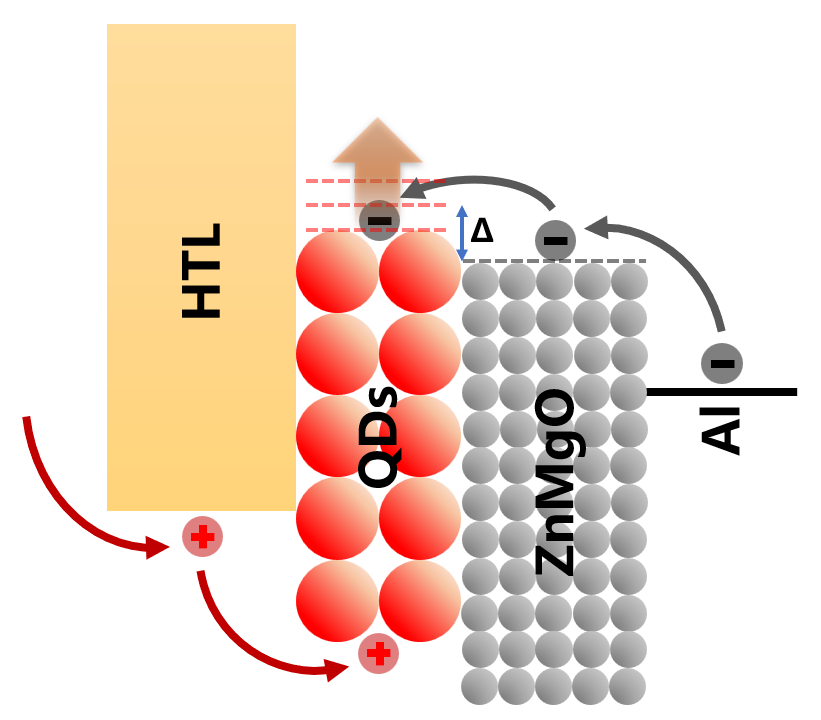
\includegraphics[width=.6\textwidth]{QD123.png}
	\caption{不同波长QDs对应的能级结构变化示意图。}
	\label{fig:QD123}
\end{figure}

在第二章第三节“\nameref{2.3}”中我们简单说了Bleaching信号强度与量子点活性层中载流子浓度呈正相关,而Stark位移信号主要反映器件内部空间电场强度分布特征,其幅值可通过相邻载流子注入层的浓度梯度进行表征。在正向偏置条件下,Bleaching信号与Stark信号表现出协同演化特性:随着外置电压升高,各功能层的电势差增大导致局域电场强度增加(对应Stark信号增强),同时载流子注入效率提升使各活性层载流子浓度升高(对应Bleaching信号增强)。值得注意的是,相邻电荷传输层载流子浓度的非对称积累会通过界面极化效应显著改变量子点层的有效电场强度,而量子点层内部载流子浓度的增加又会通过空间电荷效应调制界面电势分布。这种载流子浓度-电场强度间的动态耦合机制,构成了Bleaching效应与Stark效应相互增强的正反馈关系。除此之外,改变QDs的波长也会影响电激发瞬态吸收光谱,下面我们可以简单解释下。图\ref{fig:QD123}展示了HTL-QDs-ETL的能级结构图,其中ETL为ZMO纳米粒子。当量子点发射波长蓝移时,带隙将增大,如果我们固定QDs的价带顶(VBM)不变,那么此时变化的只有QDs的导带底(CBM),QDs的CBM将上升,如图\ref{fig:QD123}中QDs层的红色虚线所示,那么电子的注入势垒$\Delta$变大。我们知道,电子隧穿概率可以表示为$T=\eu^{-\frac{2}{\hbar}\int \sqrt{2m_e^*\Delta(x)}\dif x}$,因此,电子更难注入QDs层将导致氧镁锌ETL层内电子的相对数目增加,故ZMO层的Bleaching信号应该呈现增强的趋势,而QDs层两侧HTL空穴相对数目可以认为变化不大而ETL的电子相对数目增加,故作用在QDs层的电场效应将增强,所以QDs的Stark信号应该呈现增强的趋势。

下面我们将用实验结果证明我们上面的说法。我们首先选用CdZnSe作为量子点层的QD-LED器件,其EETA的主要信号来源于电子传输层/量子点层/空穴传输层——ZMO/CdZnSe/PFDF。我们取了CdZnSe波长为477nm的一份蓝色器件,测量了其在不同电压下的EETA稳态信号,如图\ref{fig:CZS-V}所示,我们将其中的信号划分了归属,下面我们默认蓝色背景部分对应ZMO,绿色背景部分对应空穴传输层,黄色背景部分对应量子点层,Bleaching信号用紫色箭头或标记表示,Stark信号用黄色箭头或标记表示。
\begin{figure}[ht]
	\centering
	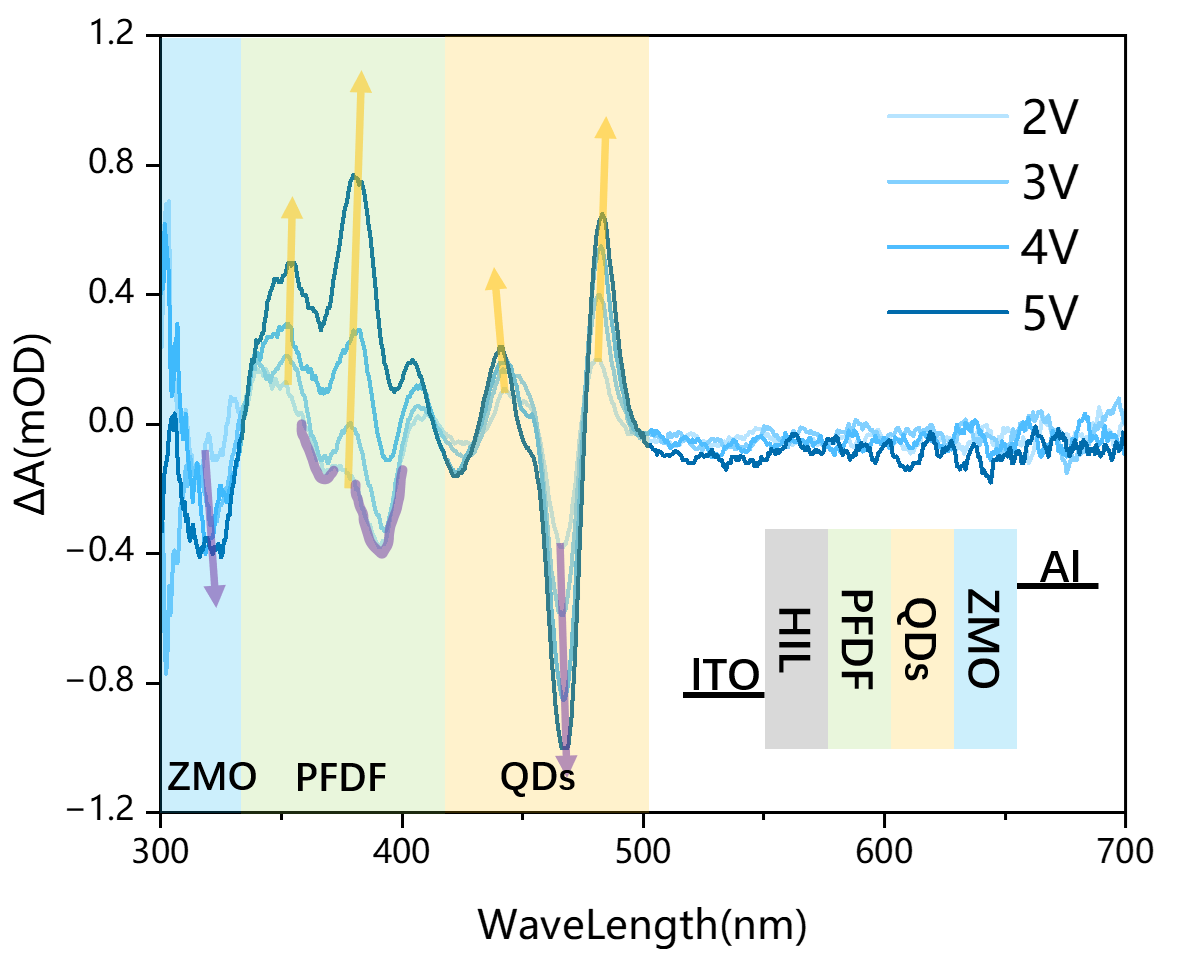
\includegraphics[width=.8\textwidth]{CZS-V.png}
	\caption{不同电压下的CdZnSe量子点器件的EETA稳态信号。}
	\label{fig:CZS-V}
\end{figure}

下面我们说明为什么我们能这样确定信号归属。首先,量子点层CdZnSe波长为477nm,很明显,在477nm附近,我们可以看到一个明显的-$\Delta$A峰,而ZMO和PFDF的吸收峰不在此附近,故该负信号只可能是CdZnSe(QDs)的Bleaching吸收峰,而在477nm的零点之上,存在一个“M”形峰,这是CdZnSe(QDs)的Stark信号,随着电压的增大,这两个信号都随之增强。其中Bleaching信号的增加表明注入QDs的电子数目在随着电压的增大而增加,Stark信号的增强是由于外加电压的增大导致QDs层的分压增大,电场效应增强,量子点能级发生更显著的Stark偏移。PFDF的信号一般在375nm附近,且具有明显的Stark效应,对应着绿色背景范围的区域,我们可以看到在2V正向偏置下,PFDF存在一个双峰Bleaching信号(紫色标记,1个大概在375nm,另一个大概在390nm),随着电压的增大,电场效应增强,我们用两个黄色箭头标记出了“M”形Stark信号的变化趋势。该器件的信号除了PFDF和QDs外只有ZMO会贡献信号,故之前范围内的Bleaching信号只能归属于ZMO,同时,我们可以看到该部分几乎不存在Stark信号,而Bleaching信号也随着电压增大而增大。整体上看,随着外加电压的增大,ZMO中电子相对数目增加,且由于各个功能层的分压增大,电子更容易从ZMO层注入QDs层,而PFDF的空穴相对数量似乎没什么变化,假定空穴注入层的空穴相对数目没什么变化,则作用在PFDF层的电场由于QDs层电子相对数目的增多而增强,PFDF层的Stark效应增强,类似的,由于ZMO层的电子相对数目增加,导致了QDs层的Stark效应增强,因此表现出图\ref{fig:CZS-V}中的电激发瞬态吸收光谱。
\begin{figure}[ht]
	\centering
	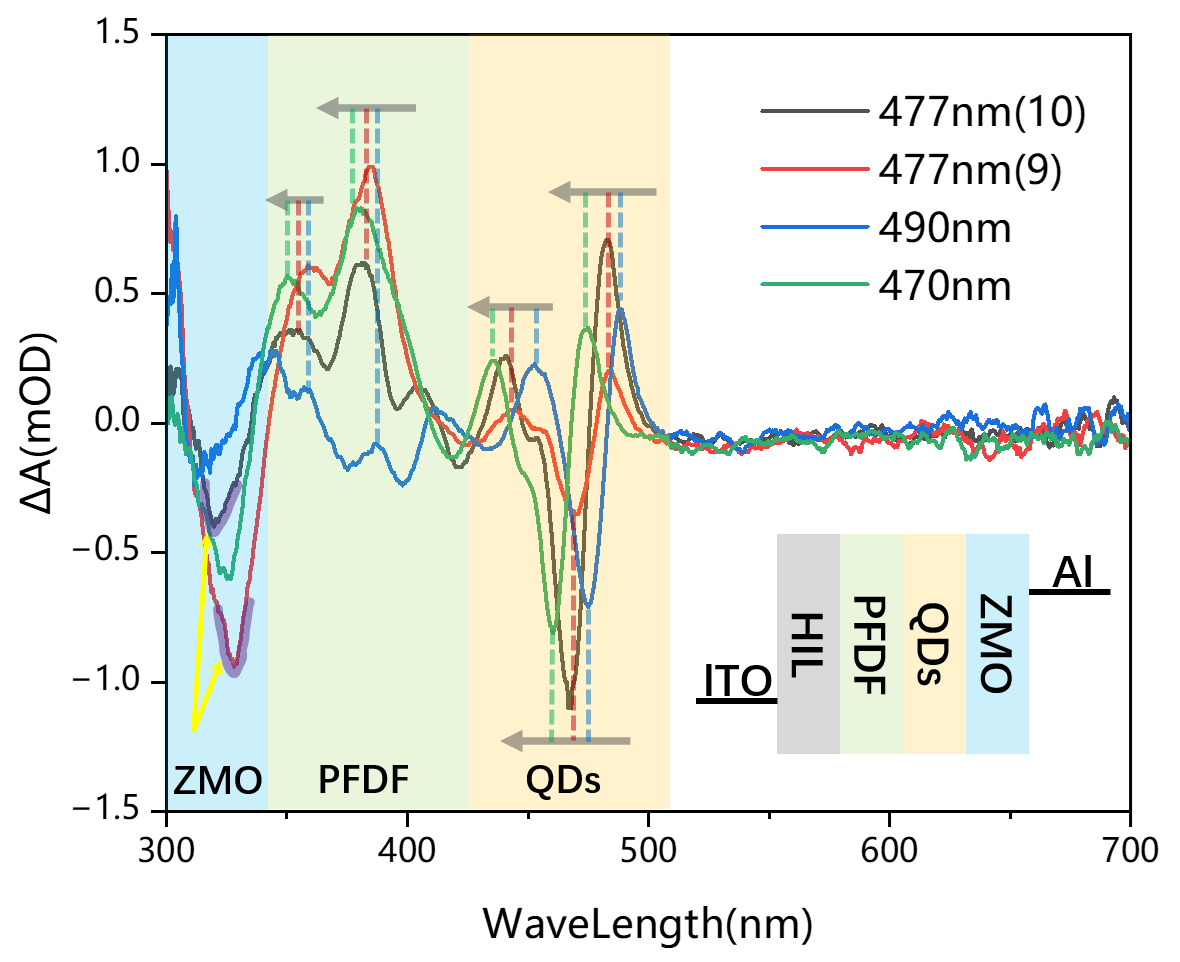
\includegraphics[width=.8\textwidth]{CZS-L.png}
	\caption{不同波长CdZnSe量子点器件的EETA稳态信号。}
	\label{fig:CZS-L}
\end{figure}

然后,我们测量了QDs波长从450nm到495nm的相同结构的CdZnSe QD-LED器件,在5V正向偏置下测量其EETA光谱,并取了其中几组比较有代表性的光谱信号展示在图\ref{fig:CZS-L}中。可以看到,对于其中490nm、470nm和477nm的10号器件这三组结果比较符合我们在本节开头的论述。QDs的信号变化基本对应着CdZnSe量子点的波长变化,而且PFDF的信号表现出和QDs相同的变化趋势,我们可以认为PFDF的Stark信号来源自量子点层,这进一步论证了我们上面简化模型是适用的,由于QDs层相对电子数目的增多导致了作用在PFDF的电场效应增强,Stark效应更加明显。不过要注意的是,对于477nm的9号器件相对于10号器件的相对异常的信号,可以认为是由于ZMO层相对于PFDF和QDs层的厚度差异导致的,可以看到477nm的第9组样品的ZMO和PFDF信号远高于其他组,但QDs信号最小,说明该组的ZMO层和PFDF层的相对厚度更大,那么其中载流子聚集程度和各种效应也会相应的增大,导致了信号强度的增强,然后ZMO的Bleaching信号红移还可能与ZMO纳米粒子的粒径大小和Mg的掺杂浓度差异有关。
\begin{figure}[ht]
	\centering
	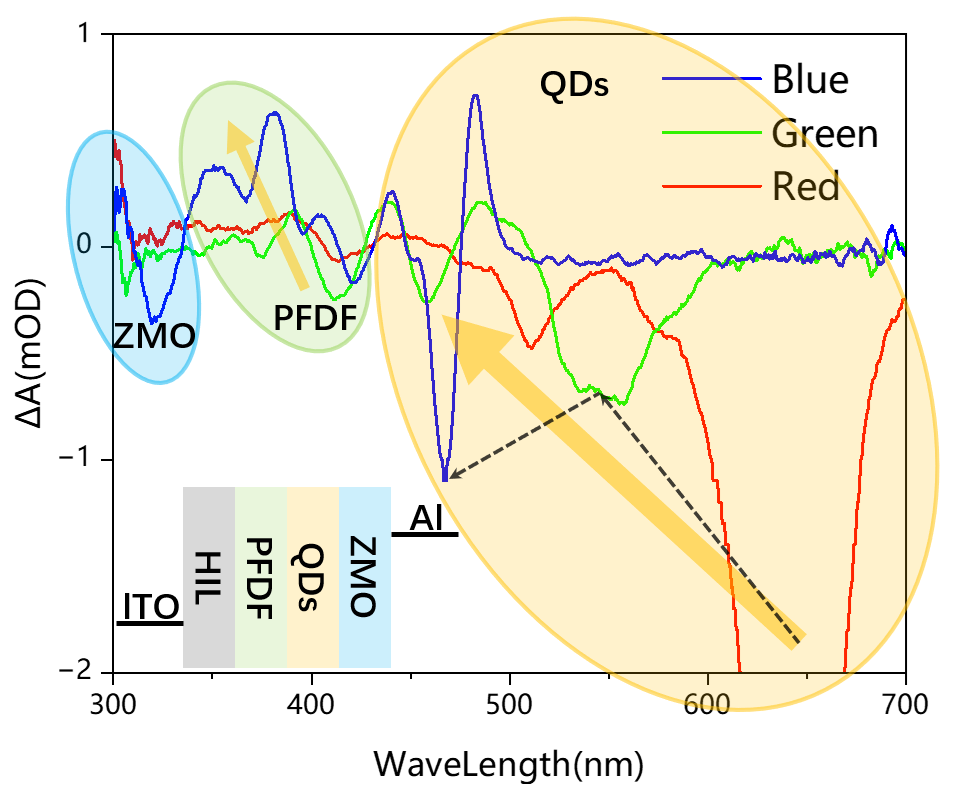
\includegraphics[width=.8\textwidth]{CZS-RGB.png}
	\caption{红绿蓝CdZnSe量子点器件的EETA稳态信号。}
	\label{fig:CZS-RGB}
\end{figure}

接着,我们又对比了红绿蓝三色的同结构CdZnSe QD-LED器件(图\ref{fig:CZS-RGB}),这里同样选取了5V的正向偏置,其中蓝色器件选用的是图\ref{fig:CZS-L}中477nm的10号器件。可以看出,QDs层和PFDF层信号的变化趋势同\ref{fig:CZS-L},对于ZMO层,信号强度从蓝到绿到红逐渐减弱,特别是红色器件,基本看不到Bleaching信号,说明对于该结构的红色器件,ZMO层中几乎不存在电子,电子的注入效率非常强,同时PFDF的信号也非常弱,说明对于此器件电子的泄露也少,二者共同导致了QDs器件非常强的Bleaching信号,这也是为什么红色器件的效率是最好的。
\begin{figure}[ht]
	\centering
	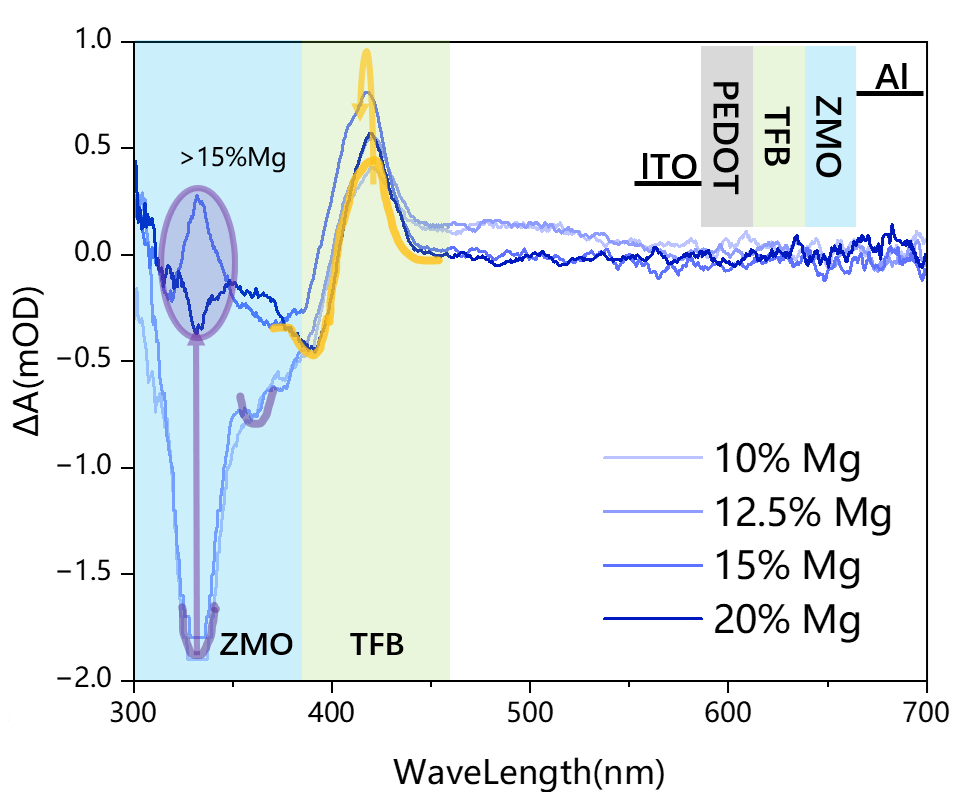
\includegraphics[width=.8\textwidth]{Mg-4.png}
	\caption{不同Mg掺杂浓度下的无量子点器件的EETA稳态信号。}
	\label{fig:Mg-4}
\end{figure}

目前,高性能QD-LED器件所选用的ZMO电子传输层,其中Mg掺杂通常在10\%时器件性能最好,随着Mg掺杂浓度的增加,实际上ZMO的载流子迁移率是在下降的,当Mg掺杂浓度超过20\%后,其迁移率将下降到一个非常低的级别,对于器件性能会造成非常巨大的影响,通常性能下降可能会超过20\%。为研究Mg掺杂浓度可能的影响,接下来我们选用了无量子点的器件,具体结构为ITO/PEDOT/TFB/ZMO/Al,对应阳极/空穴注入层/空穴传输层/电子传输层/阴极,其中PEDOT无EETA信号,故电激发瞬态吸收光谱中的信号主要来自ZMO和TFB,我们知道TFB的信号峰位一般在420nm左右,再结合上面几乎可以确定的ZMO峰位大概在320nm左右,我们可以很大的确定TFB和ZMO的EETA信号位置,下面我们用蓝色背景部分表示ZMO信号,绿色背景位置表示TFB信号。我们选取了不同Mg掺杂浓度下的器件,在4V正向偏置下测量EETA,结果如图\ref{fig:Mg-4}所示,我们用黄色标记了TFB的信号形状。如图\ref{fig:Mg-4},TFB应该表现出一个一阶Stark信号,并且随着Mg掺杂浓度的提高表现出先提高后减弱的趋势。而对于ZMO的信号,我们注意到在10\%和12.5\%Mg掺杂浓度下其Bleaching信号较强,并且应该是存在330nm和360nm两个Bleaching峰位的,其中330nm的这个Bleaching信号与之前的结果应该是一致的,比较令人疑惑的是在360nm处的小峰,我们有两个猜想:首先,可能ZMO有多个能态,5V正向偏置下应该大部分电子处于高能级,对应330nm的峰,而360nm的峰则对应低能级;还有一种可能是掺杂Mg的氧化锌纳米粒子中不完全以ZMO的形式,可能有部分未受影响而表现出原本的ZnO,不过该部分肯定是极少数,所以对应的Bleaching信号的要弱得多,这也正好符合掺Mg后吸收峰蓝移的结果,因此330nm的高峰对应ZMO,而330nm的低峰对应ZnO。此外,在Mg掺杂达到15\%和20\%后,330nm峰位的$\Delta$A出现了异常的行为,同时360nm处的峰消失,对于此,我们暂时还没有结论。
\begin{figure}[ht]
	\centering
	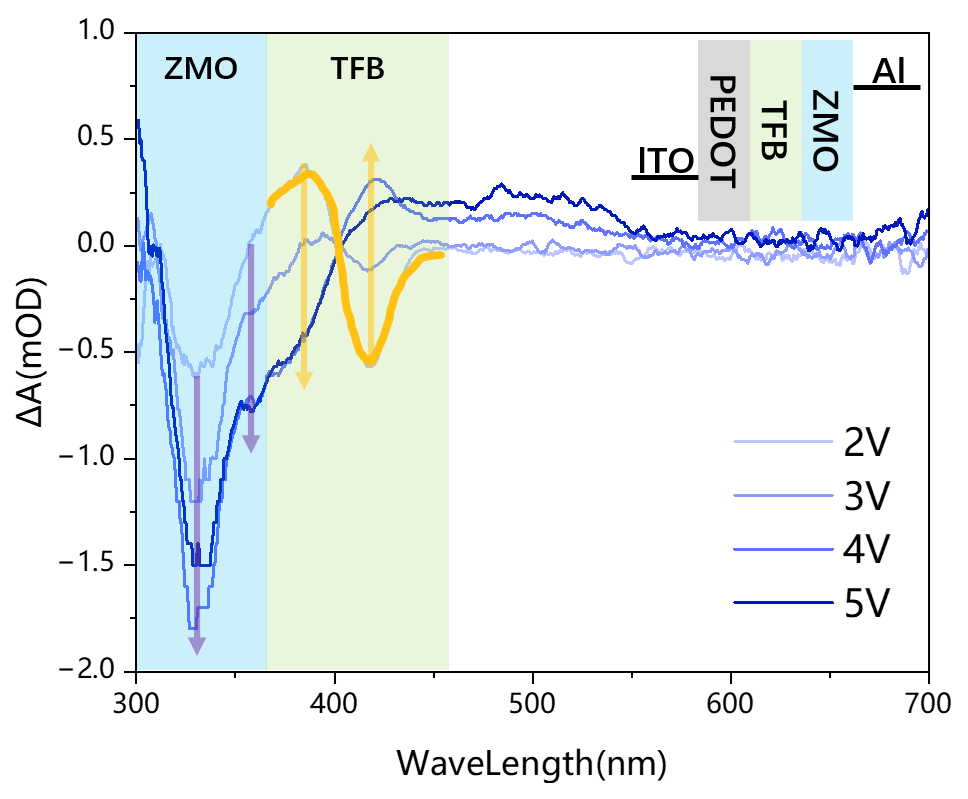
\includegraphics[width=.8\textwidth]{Mg-V.png}
	\caption{不同电压的无量子点器件的EETA稳态信号。}
	\label{fig:Mg-V}
\end{figure}

我们再选取10\%Mg掺杂的器件,测量了其在不同正向电压偏置下的EETA稳态光谱,如图\ref{fig:Mg-V}所示,可以看到,TFB的信号主要包含一个Bleaching信号和一个Stark信号,而随着电压的增大,电场效应增强,该信号因为Stark信号的增大而实现了反转。对于ZMO信号而言,其几乎只有Bleaching信号,且随着电压增大,Bleaching信号的峰位几乎无变化,而强度在增强,这是因为随着电压增大,各层级电子相应会变多,Bleaching信号随之增强,而在5V时,ZMO和TFB的信号相对于4V的情况都出现了一定程度的减弱,该趋势是几乎是同步的,说明应该是TFB和ZMO共同作用的结果,最大可能是在而这界面上行为发生了变化,推测可能与TFB和ZMO的势垒有关,可能5V时能量基本超过了该势垒,载流子几乎无阻碍越过势垒直接在界面辐射复合,导致各层的载流子数目产生了一定程度的下降。

\section{本章小结}
本章我们先简单介绍了ZnO纳米粒子,包括结构、缺陷、合成和光谱信息以及作为电子传输层的优劣势。我们也说明了目前ZnO类电子传输层的还存在的问题,特别点出对于ZnO在QD-LED中的机理研究尚且不完善,这将是实现QD-LED商业化的一个重要难题。接着,我们用隧穿模型简单介绍了只改变QDs波长对于整个器件的影响。在实验部分,我们选取了不同波长的CdZnSe器件以及为了单独观察不同Mg掺杂的影响而设计的无量子点器件进行EETA测量,并对结果进行了初步的分析,不过由于样品测试数目偏少以及缺少ZnO作为电子传输层的器件的对照,对于ZMO电子传输层的EETA稳态信号的了解基本只能请确定其位置大概在320-330nm左右,且主要是Bleaching信号,但基本没有获取到关于ZMO的其他有用信息。不过依然有很多有趣的现象值得之后去进一步研究。后面可能需要更多的器件帮助去我们进一步了解ZMO/ZnO,特别是我们还缺少载流子注入动力学的有效信息,这些基本是后面的工作了。